\chapter{Assignment-Complex Numbers}
\section{MCQ}
\begin{enumerate}
	\item $\left. \right. $
	\begin{answer}
		\begin{align*}
	\frac{1+i \sqrt{3}}{\sqrt{3}+i}&=\frac{(1+i \sqrt{3})(\sqrt{3}-i)}{(\sqrt{3}+i)(\sqrt{3}-i)}=\frac{2 \sqrt{3}+2 i}{4}=\frac{\sqrt{3}}{2}+\frac{1}{2} i\\
\intertext{	Since both the real and complex parts are greater than zero, hence the argument is the acute angle given by $\tan ^{-1}\left|\frac{\frac{1}{2}}{\frac{\sqrt{3}}{2}}\right|=\tan ^{-1} \frac{1}{\sqrt{3}}=\frac{\pi}{6}$}
		\end{align*}
		So the correct answer is \textbf{Option (c)}
	\end{answer}
\item $\left. \right. $	
	\begin{answer}
		\begin{align*}
		a+i b&=\frac{1-i x}{1+i x} \Rightarrow a-i b=\frac{1+i x}{1-i x}\\
		\therefore \quad(a+i b)(a-i b)&=\frac{1-i x}{1+i x} \cdot \frac{1+i x}{1-i x} \Rightarrow a^{2}+b^{2}=\frac{1+x^{2}}{1+x^{2}}=1
		\end{align*}
		So the correct answer is \textbf{Option (a)}
	\end{answer}
\item $\left. \right. $	
	\begin{answer}
		\begin{align*}
		|z|=\sqrt{(1-\cos \theta)^{2}+\sin ^{2} \theta}=\sqrt{2-2 \cos \theta}=\sqrt{4 \sin ^{2} \frac{\theta}{2}}=2\left|\sin \frac{\theta}{2}\right|
		\end{align*}
		So the correct answer is \textbf{Option (c)}
	\end{answer}
\item $\left. \right. $		
	\begin{answer}
		\begin{align*}
		|z|=\frac{1}{|2+3 i|^{2}}=\frac{1}{\left(\sqrt{2^{2}+3^{2}}\right)^{2}} \quad|z|=\frac{1}{13}
		\end{align*}
		So the correct answer is \textbf{Option (a)}
	\end{answer}
\item $\left. \right. $		
	\begin{answer}
		\begin{align*}
		x_{1} \cdot x_{2} \cdot x_{3} \ldots .&\text{ to infinity }=\left(\cos \frac{\pi}{2}+i \sin \frac{\pi}{2}\right)\left(\cos \frac{\pi}{2^{2}}+i \sin \frac{\pi}{2^{2}}\right)\left(\cos \frac{\pi}{2^{3}}+i \sin \frac{\pi}{2^{3}}\right) \ldots \infty\\
		&=\cos \left(\frac{\pi}{2}+\frac{\pi}{2^{2}}+\frac{\pi}{2^{3}}+\ldots\right)+i \sin \left(\frac{\pi}{2}+\frac{\pi}{2^{2}}+\frac{\pi}{2^{3}}+\ldots\right)=\cos \left(\frac{\frac{\pi}{2}}{1-\frac{1}{2}}\right)+i \sin \left(\frac{\frac{\pi}{2}}{1-\frac{1}{2}}\right)\\
		&=\cos \pi+2 i \sin \pi=-1
		\end{align*}
		So the correct answer is \textbf{Option (c)}
	\end{answer}
\item $\left. \right. $		
	\begin{answer}
		\begin{align*}
		|z|&=\left|z-\frac{4}{z}+\frac{4}{z}\right| \leq\left|z-\frac{4}{z}\right|+\left|\frac{4}{z}\right|
		\intertext{Using triangle in equinity}
		\Rightarrow \quad&|z| \leq 2+\frac{4}{|z|} \quad\text{ since } \left|z-\frac{4}{z}\right|=2\\
		&\Rightarrow \quad|z|^{2}-2|z|-4 \leq 0 \Rightarrow(|z|-1+\sqrt{5})(|z|-1-\sqrt{5}) \leq 0 \Rightarrow(1-\sqrt{5}) \leq|z| \leq 1+\sqrt{5}\\
		\text{Thus }&\text{the maximum value of }\text{$|z|$ is $1+\sqrt{5}$}
		\end{align*}
		So the correct answer is \textbf{Option (b)}
	\end{answer}
\item $\left. \right. $		
\begin{answer}
	\begin{align*}
	&1+\sum_{k=0}^{14}\left\{\cos \frac{(2 k+1) \pi}{15}+i \sin \frac{(2 k+1) \pi}{15}\right\}\\
	&=1+\sum_{k=0}^{14} e^{i \frac{(2 k+1) \pi}{15}}=1+\sum_{k=0}^{14} \alpha^{2 k+1}\qquad
\text{	where }\alpha=e^{i \frac{\pi}{15}}\\
&=1+\left(\alpha+\alpha^{3}+\alpha^{5}+\ldots \alpha^{29}\right)=1+\alpha\left(\frac{1-\left(\alpha^{2}\right)^{15}}{1-\alpha^{2}}\right)\\
&=1+\alpha\left(\frac{1-\alpha^{30}}{1-\alpha^{2}}\right)=1+\alpha\left(\frac{1-1}{1-\alpha^{2}}\right)=1 \quad\left[\right.\text{ since }\left.\quad \alpha^{30}=e^{\mathrm{i} 2 \pi}=1\right]
	\end{align*}
	So the correct answer is \textbf{Option (c)}	
\end{answer}	
\item $\left. \right. $
\begin{answer}
	\begin{align*}
	\text{Let }z&=x+i y,\text{ then}\\
	|z+4|^{2}-|z-4|^{2}&=8 \Rightarrow 4 \operatorname{Re}(4 z)=8
\intertext{	where $\operatorname{Re}(4 z)$ is the real part of the complex number $4 z$}
\Rightarrow \quad \operatorname{Re}(z)&=\frac{1}{2} \Rightarrow x=\frac{1}{2},\text{ which is a straight line parallel to the $y$-axis.}
	\end{align*}
	So the correct answer is \textbf{Option (b)}
\end{answer}	
\item $\left. \right. $	
	\begin{answer}
		\begin{align*}
		\intertext{we have}
		\left|\begin{array}{ccc}6 i & -3 i & 1 \\ 4 & 3 i & -1 \\ 20 & 3 & i\end{array}\right|&=\left|\begin{array}{ccc}6 i & 0 & 1 \\ 4 & 0 & -1 \\ 20 & 0 & i\end{array}\right| \quad\left(\right.\text{ Applying }C_{2} \rightarrow C_{2}+3 i C_{2} )\\
		&=0=0+0 i\\
		\therefore x&=0, y=0
		\end{align*}
		So the correct answer is \textbf{Option (d)}
	\end{answer}
\item $\left. \right. $		
\begin{answer}
	\begin{align*}
	&\text{we have: }\frac{z-1}{z+1}\text{ is purely imaginary}\\
	&\Rightarrow \quad\text{ argument of }\frac{z-1}{z+1}\text{ is }\pm \frac{\pi}{2} \Rightarrow \arg \left(\frac{\mathrm{z}-1}{\mathrm{z}+1}\right)=\pm \frac{\pi}{2}\\
	&\Rightarrow \quad z\text{ lies on a circle having $(1,0)$ and $(-1,0)$ as the end point of a diameter.}\\
	&\Rightarrow \quad z\text{ lies on a circle with centre at the origin and radius are unit}\\
	&\Rightarrow \quad z\text{ lies on }|z|=1 \Rightarrow|z|=1
	\end{align*}
		So the correct answer is \textbf{Option (a)}
\end{answer}
	\item $\left. \right. $
\begin{answer}
	\begin{align*}
	\int_{0}^{\pi} \frac{2 d \theta}{R-\cos \theta}&=\frac{1}{2} \int_{0}^{2 \pi} \frac{2 d \theta}{R-\cos \theta}=\int_{0}^{2 \pi} \frac{d \theta}{R-\cos \theta}\\
	z&=e^{i \theta} \Rightarrow d z=i e^{i \theta} d \theta=i z d \theta \Rightarrow d \theta=\frac{d z}{i z} \\
	\therefore \int_{0}^{\pi} \frac{2 d \theta}{R-\cos \theta}&=\oint_{c} \frac{d z / i z}{R-\frac{1}{2}\left(z+z^{-1}\right)}=\oint_{C} \frac{d z / i z}{R-\frac{1}{2}\left(\frac{z^{2}+1}{z}\right)}=\oint_{C} \frac{d z / i z}{\frac{2 R z-\left(z^{2}+1\right)}{2 z}}\\
	&=-\frac{2}{i} \oint_{c} \frac{d z}{z^{2}-2 R z+1}\hspace{2cm}
	\text{	where $C$; unit circle}\\
	\text{Poles are }&: z^{2}-2 R z+1=0\\
	\Rightarrow z&=\frac{-(-2 R) \pm \sqrt{4 R^{2}-4 \times 1 \times 1}}{2 \times 1} \quad \Rightarrow z=\frac{2 R \pm \sqrt{4 R^{2}-4}}{2} \quad \Rightarrow z=\frac{2 R \pm 2 \sqrt{R^{2}-1}}{2}\\
	&=R \pm \sqrt{R^{2}-1}\\
	z_{1}&=R+\sqrt{R^{2}-1} z_{2}=R-\sqrt{R^{2}-1} \quad(\text{ inside }C)\\
	\operatorname{Res}\left(z=z_{2}\right)&=\lim _{z \rightarrow z_{2}}\left(z-z_{2}\right) \frac{1}{\left(z-z_{1}\right)\left(z-z_{2}\right)}\\
	&=\frac{1}{z_{2}-z_{1}}=\frac{1}{R-\sqrt{R^{2}-1-R-\sqrt{R^{2}-1}}}=\frac{-1}{2 \sqrt{R^{2}-1}}\\
	\therefore \int_{0}^{\pi} \frac{2 d \theta}{(R-\cos \theta)}&=\frac{-2}{i} \times 2 \pi i \times \frac{-1}{2 \sqrt{R^{2}-1}}=\frac{2 \pi}{\sqrt{R^{2}-1}}
	\end{align*}
	So the correct answer is \textbf{Option (b)}
\end{answer}
\item $\left. \right. $
\begin{answer}
	\begin{align*}
	\oint_{C} \frac{d z}{\left(1+z^{2}\right)^{2}}&=\int_{-\infty}^{+\infty} \frac{d x}{\left(1+x^{2}\right)^{2}}+\int_{\Gamma} \frac{d z}{\left(1+z^{2}\right)^{2}}\\
	\text{	poles, }1+z^{2}&=0 \quad z=\pm i\text{ of order $2 \quad z=i$ is inside } c\\
	\therefore \operatorname{Res}(z=i)&=\lim _{z \rightarrow i} \frac{1}{\lfloor} \frac{d}{d z}\left[(z-i)^{2} \frac{1}{(z-i)^{2}(z+i)^{2}}\right]=\lim _{z \rightarrow i} \frac{-2}{(z+i)^{3}}=\frac{1}{4 i}\\
	\oint_{C} \frac{d z}{\left(1+z^{2}\right)^{2}}&=2 \pi i \times \frac{1}{4 i}=\frac{\pi}{2}\text{ also }\int_{\Gamma} \frac{d z}{\left(1+z^{2}\right)^{2}}=0\\
	\therefore \int_{-\infty}^{+\infty} \frac{d x}{\left(1+x^{2}\right)^{2}}&=\frac{\pi}{2}
	\end{align*}
	So the correct answer is \textbf{Option (a)}
\end{answer}
\item $\left. \right. $
\begin{answer}
	\begin{align*}
	\frac{\sin 3 z}{z^{2}}&=\frac{1}{z^{2}}\left[3 z-\frac{(3 z)^{3}}{\lfloor 3}+\ldots\right]=\frac{3}{z}-\frac{9}{2} z+\ldots\\
	\text{Residue }&=3\\
	\therefore \oint_{C} \frac{\sin 3 z}{z^{2}} d z&=2 \pi i \times 3=6 \pi i
	\end{align*}
	So the correct answer is \textbf{Option (a)}
\end{answer}
\item $\left. \right. $
\begin{answer}
	\begin{align*}
	&=\frac{1}{2} \int_{0}^{2 \pi} \frac{1+\cos 2 \theta}{5-4 \cos \theta} d \theta=R \cdot P \cdot \frac{1}{2} \int_{0}^{2 \pi} \frac{1+e^{i 2 \theta}}{5-4 \cos \theta} d \theta\\
	\int_{0}^{2 \pi} \frac{1+e^{i 2 \theta}}{5-4 \cos \theta} d \theta&=\oint_{c} \frac{\left(1+z^{2}\right) d z / i z}{5-\frac{4}{2}\left(z+\frac{1}{z}\right)}\\
	&=\oint_{c} \frac{\left(1+z^{2}\right) / i z}{5-2\left(\frac{z^{2}+1}{z}\right)} d z=\oint_{c} \frac{\left(1+z^{2}\right) / i z}{\frac{5 z-2 z^{2}-2}{z}} d z=\frac{-1}{i} \oint_{c} \frac{\left(1+z^{2}\right) d z}{2\left(z^{2}-\frac{5}{2} z+1\right)}\\
	\text{Poles are: }z^{2}-\frac{5}{2} z+1&=0\\
	\Rightarrow z&=\frac{-\left(-\frac{5}{2}\right) \pm \sqrt{\left(-\frac{5}{2}\right)^{2}-4}}{2}\\
	&=\frac{\frac{5}{2} \pm \sqrt{\frac{25}{4}-4}}{2}=\frac{\frac{5}{2} \pm \frac{1}{2} \sqrt{25-16}}{2}=\frac{5 \pm 3}{4}\\
	z_{1}&=\frac{5+3}{4}=\frac{8}{4}=2, z_{2}=\frac{5-3}{4}=\frac{2}{4}=\frac{1}{2}\text{ and }z_{2}=\frac{1}{2}\text{ is inside $c$.}\\
	\therefore \operatorname{Res}\left(z=\frac{1}{2}\right)&=\lim _{z \rightarrow \frac{1}{2}}\left(z-\frac{1}{2}\right) \frac{\left(1+z^{2}\right)}{(z-2) 2\left(z-\frac{1}{2}\right)}=\frac{1+1 / 4}{(1 / 2-2) 2}=\frac{-5}{12}\\
	\therefore \int_{0}^{2 \pi} \frac{1+e^{i 2 \theta}}{5-4 \cos \theta}&=\frac{-1}{i} \times 2 \pi i \times \frac{-5}{12}=\frac{10 \pi}{12}\\
	\therefore \int_{0}^{2 \pi} \frac{\cos ^{2} \theta d \theta}{5-4 \cos \theta}&=\frac{1}{2} \times \frac{10 \pi}{12}=\frac{5 \pi}{12}
	\end{align*}
	So the correct answer is \textbf{Option (c)}
\end{answer}
\item $\left. \right. $
\begin{answer}
	\begin{align*}
	&=R \cdot P \cdot \int_{0}^{2 \pi} \frac{e^{i \theta}}{13-12 \cos 2 \theta} d \theta\\
	&=\oint_{c} \frac{z \frac{d z}{i z}}{13-\frac{12}{2}\left(z^{2}+\frac{1}{z^{2}}\right)}=\frac{1}{i} \oint_{c} \frac{d z}{\frac{13 z^{2}-6\left(z^{4}+1\right)}{z^{2}}}\\
	&=\frac{1}{i} \oint_{c} \frac{d z}{13 z^{2}-6 z^{4}-6}=-\frac{1}{i} \oint_{c} \frac{z^{2} d z}{6 z^{4}-13 z^{2}+6}\\
	\text{	Poles, }&6 z^{4}-13 z^{2}+6=0\\
	\Rightarrow&\left(2 z^{2}-3\right)\left(3 z^{2}-2\right)=0\\
	\Rightarrow z&=\pm \sqrt{\frac{3}{2}}, z=\pm \sqrt{\frac{2}{3}}\\
	z&=\pm \sqrt{\frac{2}{3}}\text{ is inside $c$}
	\intertext{Applying L'Hospital's rule and simple pole formula, we get}
	\operatorname{Res}(z=\alpha)&=\lim _{z \rightarrow \alpha} \frac{(z-\alpha) z^{2}}{6 z^{4}-13 z^{2}+6}\\
	&=\lim _{z \rightarrow \alpha} \frac{(z-\alpha) \cdot 2 z+z^{2}}{24 z^{3}-26 z}=\lim _{z \rightarrow \alpha} \frac{2(z-\alpha)+z}{24 z^{2}-26}\\
	&=\lim _{z \rightarrow \alpha} \frac{2 z-2 \alpha+z}{24 z^{2}-26}=\lim _{z \rightarrow \alpha} \frac{3 z-2 \alpha}{24 z^{2}-26}=\frac{3 \alpha-2 \alpha}{24 \alpha^{2}-26}=\frac{\alpha}{24 \alpha^{2}-26}\\
	\operatorname{Res}\left(z=+\sqrt{\frac{2}{3}}\right)&=\frac{\sqrt{2 / 3}}{24 \times \frac{2}{3}-26}=\frac{-1}{10} \sqrt{\frac{2}{3}}\\
	\operatorname{Res}\left(z=-\sqrt{\frac{2}{3}}\right)&=\frac{-\sqrt{2 / 3}}{24 \times \frac{2}{3}-26}=\frac{+1}{10} \sqrt{\frac{2}{3}}\\
	\text{Sum of residue }&=0\\
	\therefore \int_{0}^{2 \pi} \frac{\cos \theta}{13-12 \cos 2 \theta} d \theta&=0
	\end{align*}
	So the correct answer is \textbf{Option (a)}
\end{answer}
\item $\left. \right. $
\begin{answer}
	\begin{align*}
	f(z)&=\frac{1}{z\left(z+\frac{1}{2}\right) \cos (z \pi)}\\
	\text{For }n^{t h}&\text{ order pole $\because \lim _{z \rightarrow a}(z-a)^{n} f(z)=$ finite and $\neq 0$}\\
	\text{At }z&=0\\
	\lim _{z \rightarrow 0} z f(z)&=\text{ finite }\Rightarrow z=0\text{ is a simple pole.}\\
	\text{At }z&=-\frac{1}{2}\\
	\lim _{z \rightarrow-\frac{1}{2}} \frac{\left(z+\frac{1}{2}\right)^{2}}{z\left(z+\frac{1}{2}\right) \cos z \pi}&=\lim _{z \rightarrow-\frac{1}{2}} \frac{\left(z+\frac{1}{2}\right)}{z \cos z \pi}=\lim _{z \rightarrow-\frac{1}{2}} \frac{1}{1 \cdot \cos z \pi+z \cdot \pi(-\sin z \pi)}\\
	&=\lim _{z \rightarrow-\frac{1}{2}} \frac{1}{\cos z \pi-z \pi \sin z \pi}=\frac{1}{\frac{\pi}{2}}=\frac{2}{\pi}=\text{ finite}\\
	\Rightarrow f(z)&\text{ has second order pole at }z=-\frac{1}{2}
	\end{align*}
	So the correct answer is \textbf{Option (b)}
\end{answer}
\item $\left. \right. $
\begin{answer}
	\begin{align*}
	I&=\oint_{C} \frac{\sin z}{2 z-\pi} \quad\text{ pole }\Rightarrow 2 z-\pi=0 \Rightarrow z=\frac{\pi}{2}\\
	\text{	Residue at }z&=\frac{\pi}{2} \quad \because|z|=2\text{ so it will be lies within the contour}\\
	I_{(e m g)}&=\oint_{C} \frac{e^{i z}}{2\left(z-\frac{\pi}{2}\right)}=\sum R \times 2 \pi i\\
	\operatorname{Res} \mid&=\frac{\left(z-\frac{\pi}{2}\right) e^{i z}}{2\left(z-\frac{\pi}{2}\right)}=\frac{e^{i \pi / 2}}{2}=\frac{i}{2}\text{ (taking imaginary part); Residue $=\frac{1}{2}$}\\
	\text{Now }I&=\frac{1}{2} \times 2 \pi i=\pi i
	\end{align*}
	So the correct answer is \textbf{Option (c)}
\end{answer}
\item $\left. \right. $
\begin{answer}
	\begin{align*}
	\text{Consider }&\int_{C} \frac{(\log z)^{2}}{x^{2}+1} d z\\
	\text{	Where }C&=[\varepsilon, R] \cup C_{R} \cup[-R,-\varepsilon] \cup C_{\varepsilon}\text{ is the contour depicted in figure given below,}\\
	\text{and take the branch }&|z|>0,-\pi / 2<\arg z<3 \pi / 2.
	\end{align*}
	\begin{figure}[H]
		\centering
		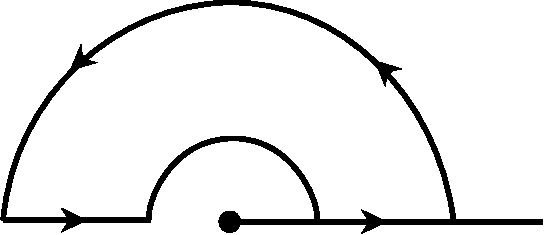
\includegraphics[height=2.3cm,width=5cm]{CN-Assignment-02}
	\end{figure}
	\begin{align*}
	\text{We have, }&\int_{\varepsilon}^{R} \frac{(\ln x)^{2}}{x^{2}+1} d x+\int_{C_{R}} \frac{(\log z)^{2}}{z^{2}+1} d z+\int_{-R}^{-\varepsilon} \frac{(\log x)^{2}}{x^{2}+1} d x+\int_{C_{\varepsilon}} \frac{(\log z)^{2}}{z^{2}+1} d z=\int_{C} \frac{(\log z)^{2}}{z^{2}+1} d z\\
	\text{Note that, }&\int_{-R}^{-\varepsilon} \frac{(\log x)^{2}}{x^{2}+1} d x=-\int_{R}^{\varepsilon} \frac{[\ln (-x)]^{2}}{x^{2}+1} d x=\int_{\varepsilon}^{R} \frac{[\log (-x)]^{2}}{x^{2}+1} d x\\
	\text{	Thus, }&\int_{\varepsilon}^{R} \frac{(\log x)^{2}}{x^{2}+1} d x+\int_{\varepsilon}^{R} \frac{[\ln (-x)]^{2}}{x^{2}+1} d x+\left(\int_{C_{R}}+\int_{C_{\varepsilon}}\right) \frac{(\log z)^{2}}{z^{2}+1} d z=2 \pi i \operatorname{Re} s_{z=i} \frac{(\log z)^{2}}{z^{2}+1}
	\intertext{Propositions 2 and 1 show that $\int_{C_{s}} \rightarrow 0$ as $\varepsilon \rightarrow 0$ and $\int_{C_{R}} \rightarrow 0$ as $R \rightarrow \infty$. Thus the above equation simplifies, and}
	2 \int_{0}^{\infty} \frac{(\ln x)^{2}}{x^{2}+1} d x&+2 i \pi \int_{0}^{\infty} \frac{\ln x}{x^{2}+1} d x-\pi^{2} \int_{0}^{\infty} \frac{d x}{x^{2}+1}=-\frac{\pi^{3}}{4}\\
	\text{But, }&\pi^{2} \int_{0}^{\infty} \frac{1}{x^{2}+1} d x=\pi^{2}\left[\tan ^{-1} x\right]_{0}^{\infty}=\frac{\pi^{3}}{2}\\
	\text{Hence, we have}&\\
	2 \int_{0}^{\infty} \frac{(\ln x)^{2}}{x^{2}+1} d x&+2 i \pi \int_{0}^{\infty} \frac{\ln x}{x^{2}+1} d x=\frac{\pi^{3}}{4}
	\intertext{whereupon, by taking the real and imaginary parts}
	\int_{0}^{\infty} \frac{(\ln x)^{2}}{x^{2}+1} d x&=\frac{\pi^{3}}{8}, \quad \int_{0}^{\infty} \frac{(\ln x)}{x^{2}+1} d x=0
	\end{align*}
	So the correct answer is \textbf{Option (c)}
\end{answer}
\item $\left. \right. $
\begin{answer}
	\begin{align*}
	z&=0\text{ is pole of order 2}\\
	\text{Pole at }z&=n \pi i\text{ lies outside the contour.}\\
	f(z)&=\frac{2}{z^{2}\left(e^{z}-e^{-z}\right)}=\frac{2}{z^{2}\left[\left(1+z+\frac{3}{2 !}+\frac{z^{3}}{3 !}+\ldots-\left(1-z+\frac{z^{2}}{2 !}-\frac{z^{3}}{3 i}\right)\right]\right.}\\
	&=\frac{2}{z^{2}\left[2 z+\frac{2 z^{3}}{3 !}+\frac{2 z^{5}}{5 !}+\ldots\right]}=\frac{2}{2 z^{3}\left[1+\frac{z^{2}}{3 !}+\frac{z^{4}}{5 !} \ldots\right]}\\
	&=\frac{1}{z^{3}}\left[1-\frac{z^{2}}{3 !}-\frac{z^{4}}{5 !}\right]=\frac{1}{z^{3}}-\frac{1}{3 ! z}-\frac{z}{5 !}\\
	\operatorname{Res}(z=0)&=\frac{-1}{6}\\
	\int_{c} \frac{d z}{z^{2} \sinh z}&=2 \pi i\left(\frac{-1}{6}\right)=\frac{-\pi i}{3}
	\end{align*}
	So the correct answer is \textbf{Option (b)}
\end{answer}
\item $\left. \right. $
\begin{answer}
	\begin{align*}
	\int_{0}^{\infty} \frac{\ln x^{2}}{\left(x^{2}+1\right)^{2}} d x&=2 \int_{0}^{\infty} \frac{\ln x}{\left(x^{2}+1\right)^{2}} d x=2 \int_{0}^{\infty} \frac{\ln z}{\left(z^{2}+1\right)^{2}} d z\\
	\text{	Let us }&\text{consider new function }f(z)=\left(\frac{\ln z}{z^{2}+1}\right)^{2},\text{ then }I=\int_{0}^{\infty}\left(\frac{\ln z}{z^{2}+1}\right)^{2} d z\\
	\text{Pole at }z&=\pm i\text{ is simple pole of second order.}\\
	\text{Residue at }z&=i\text{ is}\\
	&=\frac{d}{d z}(z-i)^{2} \frac{(\ln z)^{2}}{(z-i)^{2}(z+i)^{2}}=\frac{d}{d z} \frac{(\ln z)^{2}}{(z+i)^{2}}\\
	&=\frac{(z+i)^{2} 2(\ln z) \cdot \frac{1}{z}-(\ln z)^{2} \cdot 2(z+i)}{(z+i)^{4}}=\frac{(z+i) 2 \ln (z) \frac{1}{z}-(\ln z)^{2} \cdot 2}{(z+i)^{3}}\\
	&=\frac{(2 i) 2 \times \frac{1}{i} \ln i-(\ln i)^{2} \cdot 2}{(2 i)^{3}}=\frac{4 \frac{i \pi}{2}-\left(\frac{i \pi}{2}\right)^{2} \times 2}{-8 i}=\frac{2 \pi i+\frac{\pi^{2}}{2}}{-8 i}\\
	\left.\Rightarrow \operatorname{Res}\right|_{z=i}&=\frac{-\pi}{4}+\frac{\pi^{2}}{16} i\\
	\text{Similarly at }z&=-i ;\left.\operatorname{Res}\right|_{z=-i}=\frac{-\pi}{4}-\frac{\pi^{2}}{16} i
	\end{align*}
	\begin{figure}[H]
		\centering
		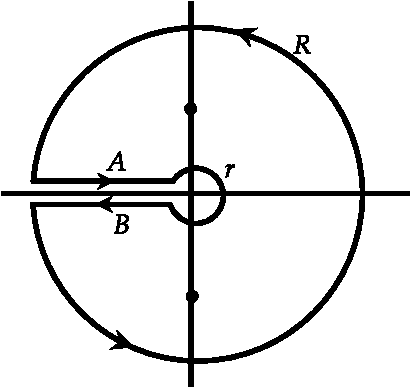
\includegraphics[height=4cm,width=4.5cm]{CN-Assignment-03}
	\end{figure}
	\begin{align*}
	I&=\int_{0}^{\infty}\left(\frac{\ln z}{z^{2}+1}\right)^{2} d z=2 \pi i\left(\frac{-\pi}{4}+\frac{\pi^{2}}{16} i-\frac{\pi}{4}-\frac{\pi^{2}}{16} i\right)=-\pi^{2} i\\
	-\pi^{2} i&=\left(\iint_{R} \int_{A} \int_{B}\right) f(z) d z=\left(\iint_{A B}\right) f(z) d z ; \iint_{A B}\text{ vanish}\\
	\text{Along path }A ; z&=-x+i \varepsilon\text{ and along path }B ; z=-x-i \varepsilon\\
	\text{Thus }-\pi^{2} i&=\left(\int_{A} \int_{B}\right) f(z) d z=-\int_{\infty}^{0}\left[\frac{\ln (-x+i \varepsilon)}{(-x+i \varepsilon)^{2}+1}\right] d x-\int_{0}^{\infty}\left[\frac{\ln (-x-i \varepsilon)}{(-x-i \varepsilon)^{2}+1}\right] d x\\
	\Rightarrow-\pi^{2} i&=\int_{0}^{\infty}\left[\frac{\ln (-x+i \varepsilon)}{(-x+i \varepsilon)^{2}+1}\right]^{2} d x-\int_{0}^{\infty}\left[\frac{\ln (-x-i \varepsilon)}{(-x-i \varepsilon)^{2}+1}\right]^{2} d x\\
	\Rightarrow-\pi^{2} i&=\int_{0}^{\infty}\left[\frac{\ln (x)+i \pi}{1+x^{2}}\right]^{2} d x-\int_{0}^{\infty}\left[\frac{\ln (x)-i \pi}{1+x^{2}}\right]^{2} d x ; \quad \varepsilon \rightarrow 0\\
	\Rightarrow-\pi^{2} i&=\int_{0}^{\infty} \frac{(\ln (x)+i \pi)^{2}-(\ln (x)-i \pi)^{2}}{\left(1+x^{2}\right)^{2}} d x=4 \pi i \int_{0}^{\infty} \frac{\ln x}{\left(x^{2}+1\right)^{2}}\\
	\Rightarrow \int_{0}^{\infty} \frac{\ln x}{\left(x^{2}+1\right)^{2}}&=\frac{-i \pi^{2}}{4 \pi i}=\frac{-\pi}{4} \Rightarrow 2 \int_{0}^{\infty} \frac{\ln x}{\left(x^{2}+1\right)^{2}}=\frac{-\pi}{2}
	\end{align*}
	So the correct answer is \textbf{Option (c)}
\end{answer}


\item $\left. \right. $
\begin{answer}
	\begin{align*}
	I&=\int_{C} \frac{z^{3} d z}{-2 z^{2}+10 z-12}=-\frac{1}{2} \int_{C} \frac{z^{3} d z}{z^{2}-5 z+6}\\
	\Rightarrow z^{2}-5 z+6&=0 \Rightarrow z^{2}-2 z-3 z+6=0 \Rightarrow z(z-2)-3(z-2)=0 \Rightarrow z=3,2\\
	2|z|&=5 \Rightarrow|z|=2.5\text{, only 2 will be inside.}\\
	Residue &=\left.(z-2) \frac{z^{3}}{(z-3)(z-2)}\right|_{z=2}=\frac{8}{2-3}=-8 \Rightarrow \int_{c} \frac{z^{3} d z}{z^{2}-5 z+6}=2 \pi i(-8)=-16 \pi i\\
	I&=\int_{C} \frac{z^{3} d z}{-2 z^{2}+10 z-12}=-\frac{1}{2} \int_{C} \frac{z^{3} d z}{z^{2}-5 z+6}=-\frac{1}{2} \times(-16 \pi i)=8 \pi i
	\end{align*}
	So the correct answer is \textbf{Option (c)}
\end{answer}
\item $\left. \right. $
\begin{answer}$\left. \right. $
	\begin{figure}[H]
		\centering
		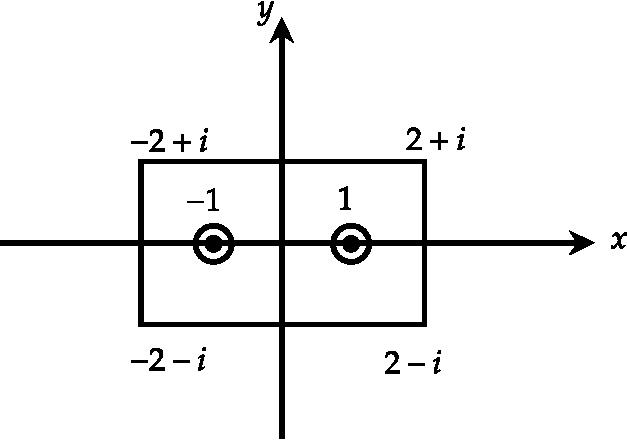
\includegraphics[height=4.1cm,width=6cm]{CN-Assignment-04}
	\end{figure}
	\begin{align*}
	f(z)&=\cos \pi z\\
	z&=\pm 1\text{ lies inside the $C$.}\\
	I&=\frac{1}{2}\left[\oint \frac{f(z) d z}{z-1}-\oint \frac{f(z)}{z+1} d z\right]\\
	I&=\frac{1}{2}[f(1) 2 \pi i-f(-1) 2 \pi i]=\pi i[\cos \pi-\cos \pi]=0
	\end{align*}
	So the correct answer is \textbf{Option (d)}
\end{answer}
\item $\left. \right. $
\begin{answer}
	\begin{align*}
	\text{Let }f(z)&=\frac{e^{i 2 z}}{z^{3}}\\
	\lim _{z \rightarrow 0}(z-0)^{3} f(z)&=\lim _{z \rightarrow 0}(z-0)^{3} \frac{e^{i 2 z}}{z^{3}}=1\text{( finite and $\neq 0) \Rightarrow z=0$ is pole of order 3 .}\\
	\text{Residue }R&=\frac{1}{2 !} \lim _{z \rightarrow 0} \frac{d^{2}}{d z^{2}}\left[(z-0)^{3} \frac{e^{i z}}{z^{3}}\right]=-2\\
	\Rightarrow \int_{-\infty}^{\infty} f(x) d x&=\pi i \Sigma R=\pi i(-2)=-2 \pi i 
	\\\Rightarrow \operatorname{Im}.\text{ Part }&=-2 \pi \Rightarrow \int_{-\infty}^{\infty} f(x) d x=-2 \pi
	\end{align*}
	So the correct answer is \textbf{Option (a)}	
\end{answer}
\item $\left. \right. $
\begin{answer}
	\begin{align*}
	\text{	Put }z&=e^{i \theta} \Rightarrow d z=i e^{i \theta} d \theta \text{where, }C:|z|=1\\
	\frac{d \theta}{5+4 \cos \theta}&=\frac{d z}{i z\left[5+\frac{4}{2}\left(z+\frac{1}{z}\right)\right]}=\frac{d z}{i\left[5 z+2 z^{2}+2\right]}=\frac{d z}{i(z+2)(2 z+1)}=\frac{d z}{2 i(z+2)(z+1 / 2)}\\
	\int_{0}^{2 \pi} \frac{d \theta}{5+4 \cos \theta}&=\frac{1}{2 i} \oint_{C} \frac{d z}{(z+2)(z+1 / 2)}\\
	\text{Poles }&\text{in the contour is }z_{0}=-1 / 2\\
	\text{Residue }&=\frac{1}{2 i} \lim _{z \rightarrow-1 / 2}(z+1 / 2) \frac{1}{(z+2)(z+1 / 2)}=\frac{1}{2 i} \frac{2}{3}\\
	\text{Thus }\int_{0}^{2 \pi} \frac{d \theta}{5+4 \cos \theta}&=2 \pi i \times \frac{1}{2 i} \frac{2}{3}=\frac{2 \pi}{3}
	\end{align*}
	So the correct answer is \textbf{Option (a)}	
\end{answer}
\item $\left. \right. $
\begin{answer}
	\begin{align*}
	\int_{-\infty}^{+\infty} \frac{x}{\left(x^{2}+1\right)\left(x^{2}+4\right)} d x&\\
	\oint_{C} \frac{z d z}{\left(z^{2}+1\right)\left(z^{2}+4\right)}&=\int_{-\infty}^{+\infty} \frac{x d x}{\left(x^{2}+1\right)\left(x^{2}+4\right)}+\int_{\Gamma} \frac{z d z}{\left(z^{2}+1\right)\left(z^{2}+4\right)}\left[\int_{\Gamma} \frac{z d z}{\left(z^{2}+1\right)\left(z^{2}+4\right)}=0\right]\\
	\text{Poles are }z^{2}+1&=0 \Rightarrow z^{2}=-1 \Rightarrow z=\pm \sqrt{-1}\\
	\therefore z&=\pm i \\
	z^{2}+4&=0 \Rightarrow z^{2}=-4 \Rightarrow z=\pm \sqrt{-4} \\
	\therefore z&=\pm 2 i\\
	\therefore z&=\pm \text { and } 2 i \text { are inside } c\\
	z&=i\text{ and $2 i$ are inside $c$}\\
	\operatorname{Res}(i)&=\lim _{z \rightarrow i} \frac{(z-i) z}{(z-i)(z+i)\left(z^{2}+4\right)}=\frac{i}{2 i \times 3}=\frac{1}{6}\\
	\operatorname{Res}(2 i)&=\lim _{z \rightarrow 2 i} \frac{(z-2 i) z}{\left(z^{2}+i\right)(z-2 i)(z+2 i)}=-\frac{1}{6}
	\intertext{Sum of residues $=0$. Hence the value of integral is zero.}
	\end{align*}
	So the correct answer is \textbf{Option (a)}
\end{answer}
\item $\left. \right. $
\begin{answer}
	\begin{align*}
	\int_{0}^{2 \pi} \frac{d \theta}{13-5 \sin \theta}&=\oint_{C} \frac{d z / i z}{13-\frac{5}{2 i}\left(z-\frac{1}{z}\right)}=\oint_{C} \frac{d z / i z}{\frac{26 i z-5 z^{2}+5}{2 i z}}\\
	&=-\oint_{C} \frac{2 d z}{5 z^{2}-26 i z-5}=-2 \int \frac{d z}{5 z^{2}-26 i z-5}\\
	\text{Poles are }&5 z^{2}-26 i z-5=0\\
	z&=\frac{26 i \pm \sqrt{-576}}{10}=\frac{26 i \pm \sqrt{576 i^{2}}}{10}=\frac{26 i \pm 24 i}{10}=5 i, \frac{i}{5}\\
	\frac{i}{5}\text{ is inside }&c\\
	\operatorname{Res}\left(z=\frac{i}{5}\right) &=\lim _{z \rightarrow i / 5}\left(z-\frac{i}{5}\right) \frac{1}{(z-5 i)(5 z-i)}=\lim _{z \rightarrow i / 5} \frac{(5 z-i)}{5(z-5 i)(5 z-i)} \\ &=\frac{1}{5(i / 5-5 i)}=\frac{5}{5(i-25 i)}=\frac{1}{-24 i}=\frac{i}{24} \\
	\therefore \int_{0}^{2 \pi} \frac{d \theta}{13-5 \sin \theta}&=-2 \pi i \times 2 \times \frac{i}{24}=\frac{\pi}{6}
	\end{align*}
	So the correct answer is \textbf{Option (d)}
\end{answer}
\item $\left. \right. $
\begin{answer}
	$\left. \right. $
	\begin{figure}[H]
		\centering
		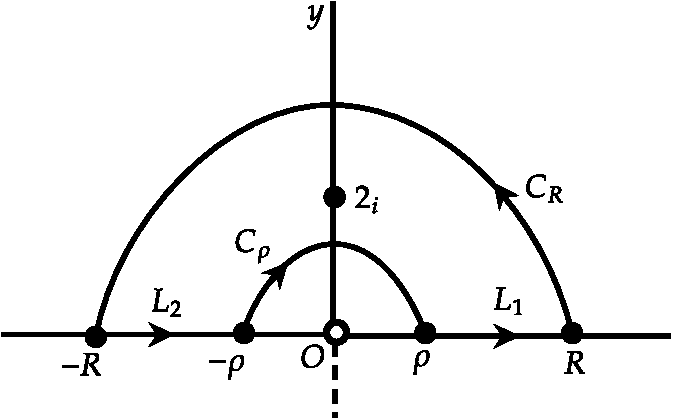
\includegraphics[height=3cm,width=5cm]{CN-Assignment-05}
	\end{figure}
	\begin{align*}
	\intertext{The solution can be derived by considering the branch}
	f(z)&=\frac{\log z}{\left(z^{2}+4\right)^{2}}\left(|z|>0,-\frac{\pi}{2}<\arg z<\frac{3 \pi}{2}\right)
	\intertext{of the multiple - valued function $(\log z) /\left(z^{2}+4\right)^{2}$. This branch, whose branch cut consists of the origin and the negative imaginary axis, is analytic everywhere in the stated domain except at the point $z=2 i$. See fig., where the same indented path and the same labels $L_{1}, L_{2}, C_{\rho}$ and $C_{R}$ as in Fig. are used. In order that the isolated singularity $z=2 i$ be inside the closed path, we require that $\rho<2<R$.}
	\intertext{	According to Cauchy's residue theorem,}
	\int_{L_{1}} f(z) d z&+\int_{C_{R}} f(z) d z+\int_{L_{2}} f(z) d z+\int_{C_{p}} f(z) d z=2 \pi i \operatorname{Res} f(z)
	\intertext{That is,}
	(2)\quad 
	\int_{L_{1}} f(z) d z&+\int_{L_{2}} f(z) d z+\int_{L_{2}} f(z) d z=2 \pi i \operatorname{Res} f(z)-\int_{C_{\rho}} f(z) d z-\int_{C_{\rho}} f(z) d z\\
	\text{	Since, }f(z)&=\frac{\ln r+i \theta}{\left(r^{2} e^{i 2 \theta}+4\right)}\left(z=r e^{i \theta}\right)
	\intertext{The parametric representations}
	(3) \quad z&=r e^{i 0}=r(\rho \leq r \leq R)\text{ and }z=r e^{i \pi}=-r(\rho \leq r \leq R)
	\intertext{for the legs $L_{1}$ and $L_{2}$, respectively, can be used to write the left - hand side of equation}
	(2) \text{as},
	\int_{L_{1}} f(z) d z-\int_{-L_{2}} f(z) d z&=\int_{\rho}^{R} \frac{\ln r}{\left(r^{2}+4\right)} d r+\int_{\rho}^{R} \frac{\ln r+i \pi}{\left(r^{2}+4\right)} d r
	\intertext{	Also, since}
	f(z)&=\frac{\phi(z)}{(z-2 i)^{2}} \text { where } \phi(z)=\frac{\log z}{(z+2 i)^{2}}
	\intertext{The singularity $z=2 i$ or $f(z)$ is a pole of order 2 , with residue}
	\phi^{\prime}(2 i)&=\frac{\pi}{64}+i \frac{1-\ln ^{2}}{32}
	\intertext{Equation (2) thus becomes}
	(4)\quad 
	2 \int_{\rho}^{R} \frac{\ln r}{\left(r^{2}+4\right)^{2}} d r&+i \pi \int_{\rho}^{R} \frac{d r}{\left(r^{2}+4\right)^{2}}=\frac{\pi}{16}(\ln 2-1)+i \frac{\pi^{2}}{32}-\int_{C_{\rho}} f(z) d z-\int_{C_{R}} f(z) d z
	\intertext{and, by equating the real parts on each side here, we find that}
	(5)\quad 
	2 \int_{\rho}^{R} \frac{\ln r}{\left(r^{2}+4\right)^{2}} d r&=\frac{\pi}{16}(\ln 2-1)-\operatorname{Re} \int_{C_{\rho}} f(z) d z-\operatorname{Re} \int_{C_{R}} f(z) d z
	\intertext{It remains only to show that}
	\lim _{\rho \rightarrow 0} \operatorname{Re} \int_{C_{\rho}} f(z) d z&=0 \text{and }\lim _{R \rightarrow \infty} \operatorname{Re} \int_{C_{R}} f(z) d z=0
	\intertext{For, by letting $\rho$ and $R$ tend to 0 and $\infty$, respectively, in equation (5), we then arrive at}
	2 \int_{0}^{\infty} \frac{\ln r}{\left(r^{2}+4\right)^{2}} d r&=\frac{\pi}{16}(\ln 2-1)
	\end{align*}
	So the correct answer is \textbf{Option (b)}
\end{answer}
\item $\left. \right. $
\begin{answer}
	\begin{align*}
	\intertext{ Consider $\oint\left(z^{p-1} / 1+z\right) d z$. Since $z=0$ is a branch points, choose $C$ as the contour of
		fig. $7.10$ where the positive real axis in the branch line and where $A B$ and $G H$ are actually coincident with the $x$ axis but are shown separated for visual purpose.}
	\text{The integral has the smile pole }z&=-1\text{ inside $C$.}\\
	\lim _{x \rightarrow-1}(z+1) \frac{z^{p-1}}{1+z}&=\left(e^{\pi i}\right)^{p-1}=e^{(p-1) \pi i}\\
	\text{Then }\oint_{C} \frac{z^{p-1}}{1+z} d z&=2 \pi i e^{(p-i) \pi i}
	\end{align*}
	\begin{figure}[H]
		\centering
		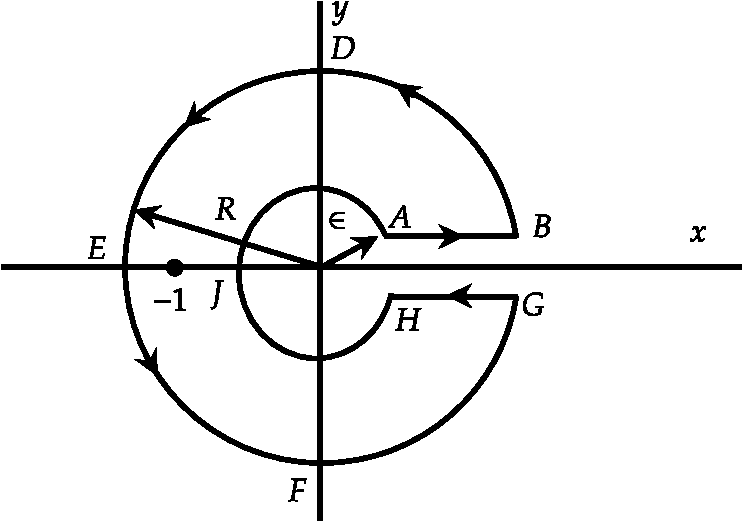
\includegraphics[height=4cm,width=6cm]{CN-Assignment-06}
	\end{figure}
	\begin{align*}
	\text{or, omitting the integrand, }&\int_{A B}+\int_{B D E F G}+\int_{G H}+\int_{H J A}=2 \pi i e^{(p-1) \pi i}
	\intertext{We thus have}
	\int_{\in}^{R} \frac{x^{p-1}}{1+x} d x+\int_{0}^{2 \pi} \frac{\left(\operatorname{Re}^{i \theta}\right)^{p-1} i \operatorname{Re}^{i \theta} d x}{1+\operatorname{Re}^{i \theta}}&+\int_{R}^{\epsilon} \frac{\left(x e^{2 \pi i}\right)^{p-1}}{1+x e^{2 \pi i}} d x+\int_{2 \pi}^{0} \frac{\left(\in e^{i \theta}\right)^{p-1} i \in e^{i \theta} d \theta}{1+\in e^{i \theta}}=2 \pi e^{(p-1) \pi i}
	\intertext{where we have used $z=x e^{2 \pi i}$ for the integral along $G H$, since the argument of $z$ is increased by $2 \pi$ in going around the circle $B D E F G$.	}
	\intertext{	Taking the limit as $\in \rightarrow 0$ and $R \rightarrow 0$ and nothing that the second and fourth integrals approach zero, we find $\int_{0}^{\infty} \frac{x^{p-1}}{1+x} d x+\int_{\infty}^{0} \frac{e^{2 \pi i(p-1)} x^{p-1}}{1+x} d x=2 \pi^{(p-1) \pi i}$}
	\text{or }&\left(1-e^{2 \pi i(p-1)} \int_{0}^{\infty} \frac{x^{p-1}}{1+x}=2 \pi i e^{(p-1) \pi i}\right)\\
	\text{So that }\int_{0}^{\infty} \frac{x^{p-1}}{1+x} d x&=\frac{2 \pi i e^{(p-1) \pi i}}{1-e^{2} \pi i(p-1)}=\frac{2 \pi i}{e^{p \pi i}-e^{-p \pi i}}=\frac{\pi}{\sin p \pi}
	\end{align*}
	So the correct answer is \textbf{Option (c)}
\end{answer}
\item $\left. \right. $
\begin{answer}
	\begin{align*}
	\oint_{c} \frac{z \cosh z \pi}{z^{4}+13 z^{2}+36} d z,|z|&=\pi\\
	z^{4}+13 z^{2}+36&=0 \Rightarrow\left(z^{2}+4\right)\left(z^{2}+9\right)=0\\
	z&=\pm 2 i, \pm 3 i\\
	\operatorname{Res}(2 i)&=\lim _{z \rightarrow 2 i} \frac{(z-2 i) z \cosh \pi z}{(z-2 i)(z+2 i)\left(z^{2}+9\right)}\\
	&=\lim _{z \rightarrow 2 i} \frac{z \cdot \cos i \pi z}{(z+2 i)\left(z^{2}+9\right)}=\frac{2 i \times \cos 2 \pi i^{2}}{(2 i+2 i)\left[(2 i)^{2}+9\right]}=\frac{2 i \times \cos (-2 \pi)}{2 \times 2 i \times 5}=\frac{\cos 2 \pi}{10}=\frac{1}{10}\\
	\operatorname{Res}(-2 i)&=\lim _{z \rightarrow-2 i} \frac{(z+2 i) z \cosh \pi z}{(z+2 i)(z-2 i)\left(z^{2}+9\right)}=\lim _{z \rightarrow-2 i} \frac{z \cos i \pi z}{(z-2 i)\left(z^{2}+9\right)}\\
	&=\frac{(-2 i) \cos [i \pi(-2 i)]}{(-2 i-2 i)\left[(-2 i)^{2}+9\right]}=\frac{(-2 i) \cos 2 \pi}{-2 \times 2 i \times 5}=\frac{1}{10}\\
	\operatorname{Res}(3 i)&=\lim _{z \rightarrow 3 i} \frac{(z-3 i) z \cosh \pi z}{(z-3 i)\left(z^{2}+4\right)(z+3 i)}=\lim _{z \rightarrow 3 i} \frac{z \cos i \pi z}{(z+3 i)\left(z^{2}+4\right)}=\frac{3 i \cos (i \pi 3 i)}{(3 i+3 i)\left[(3 i)^{2}+4\right]}\\
	&=\frac{\cos (-3 \pi)}{2(-9+4)}=\frac{1}{10}\\
	\operatorname{Res}(-3 i)&=\lim _{z \rightarrow-3 i} \frac{(z+3 i) z \cosh \pi z}{(z+3 i)(z-3 i)\left(z^{2}+4\right)}=\lim _{z \rightarrow-3 i} \frac{z \cos i \pi z}{(z-3 i)\left(z^{2}+4\right)}\\
	&=\frac{(-3 i) \cos [i \pi(-3 i)]}{(-3 i-3 i)\left[(-3 i)^{2}+4\right]}=\frac{\cos 3 \pi}{2[-9+4]}=\frac{1}{10}\\
	\therefore \oint_{c} \frac{z \cosh \pi z}{z^{4}+13 z^{2}+36} d z&=2 \pi i \times \frac{4}{10}=\frac{4 \pi i}{5}
	\end{align*}
	So the correct answer is \textbf{Option (c)}
\end{answer}	
\section{NAT}
\item $\left. \right. $		
\begin{answer}
	\begin{align*}
	\intertext{we have}
	\left(\frac{1+i}{1-i}\right)^{n}&=\left(\frac{(1+i)(1+i)}{(1-i)(1+i)}\right)^{n}=\left(\frac{(1+i)^{2}}{1-i^{2}}\right)^{n}=i^{n} .\text{ Clearly, it is real for }n=2
	\end{align*}
		So the correct answer is \textbf{2}
\end{answer}
	\item $\left. \right. $	
	\begin{answer}
		\begin{align*}
			i^{n}+i^{n+1}+i^{n+2}+i^{n+3}&=i^{n}\left(1+i+i^{2}+i^{3}\right)\\
		&=i^{n}[1+i-1-i]=0
		\end{align*}
		So the correct answer is \textbf{0}
	\end{answer}
\item $\left. \right. $		
	\begin{answer}
		\begin{align*}
		\intertext{we have}
		(\cos 3 \theta+i \sin 3 \theta)^{4}&=\cos 12 \theta+i \sin 12 \theta=(\cos \theta+i \sin \theta)^{12}\\
		(\cos 4 \theta-i \sin 4 \theta)^{5}&=\cos 20 \theta-i \sin 20 \theta=(\cos \theta+i \sin \theta)^{-20}\\
		(\cos 4 \theta+i \sin 4 \theta)^{3}&=\cos 12 \theta+i \sin 12 \theta=(\cos \theta+i \sin \theta)^{12}\\
		(\cos 5 \theta+i \sin 5 \theta)^{-4}&=\cos 20 \theta-i \sin 20 \theta=(\cos \theta+i \sin \theta)^{-20}
		\intertext{Hence the value of given expression is 1}
		\end{align*}
			So the correct answer is \textbf{1}
	\end{answer}
\item $\left. \right. $	
	\begin{answer}
		\begin{align*}
		\frac{1-i \sqrt{3}}{2}\text{ and }\frac{-1-i \sqrt{3}}{3}\text{ are cube roots}&\text{ of unity. If we denote }\frac{1-i \sqrt{3}}{2}\text{ by }\omega \text{ then }\frac{-1-i \sqrt{3}}{3}=\omega^{2}\\
\text{Hence }\left(\frac{1-i \sqrt{3}}{2}\right)^{n}+\left(\frac{-1-i \sqrt{3}}{2}\right)^{n}&=\omega^{n}+\left(\omega^{2}\right)^{n}=\omega^{6 k}+\omega^{12 k}=\left(\omega^{3}\right)^{2 k}+\left(\omega^{3}\right)^{4 k}=1+1=2
		\end{align*}
		So the correct answer is \textbf{2}
	\end{answer}
\item $\left. \right. $	
	\begin{answer}
		\begin{align*}
		z^{69}=&\left(\cos \frac{\pi}{6}+i \sin \frac{\pi}{6}\right)^{69}=\left(\cos \frac{69 \pi}{6}+i \sin \frac{69 \pi}{6}\right)=\cos \frac{23 \pi}{2}+i \sin \frac{69 \pi}{6}\\
		&=i \sin \frac{23 \pi}{2}=-i \sin \frac{\pi}{2}=-i
		\end{align*}
			So the correct answer is \textbf{$-i$}
	\end{answer}
	\section{MSQ}
\item $\left. \right. $	
\begin{answer}
	\begin{align*}
	\intertext{The magnitude of a complex number}
	z&=x+i y\text{ is given by }|z|=\sqrt{x^{2}+y^{2}}\\
	\text{hence }z&=\sqrt{4^{2}+2^{2}}=\sqrt{20}=2 \sqrt{5}\text{ units}
	\intertext{The argument is given by}
	\tan ^{-1}&\left|\frac{y}{x}\right|\text{, since both }x \& y>0\\
	\text{Hence }&\text{argument or amplitude is }z=\tan ^{-1}\left|\frac{2}{4}\right|=\tan ^{-1} \frac{1}{2}
	\end{align*}
	So the correct answers are \textbf{Option (a) and (d)}
\end{answer}
\item $\left. \right. $		
	\begin{answer}$\left. \right. $\\
		\begin{figure}[H]
			\centering
			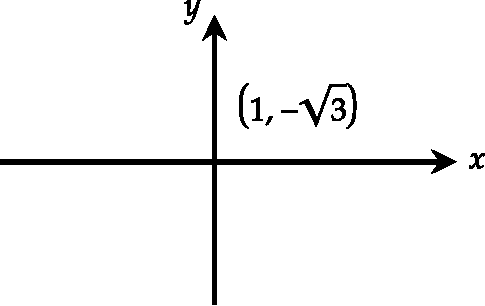
\includegraphics[height=3cm,width=5cm]{CN-Assignment-01}
		\end{figure}
		\begin{align*}
		\text{The magnitude is }|z|&=\sqrt{(1)^{2}+(-\sqrt{3})^{2}}=2\text{ units.}
		\intertext{A complex number in the complex plane is represent by a point.}
		\intertext{The real part is plotted on the $x$-axis and imaginary part on the $y$-axis. hence $z=1-\sqrt{3} i$ can be represented by a point $(1,-\sqrt{3})$ in the complex plane.}
		\end{align*}
		So the correct answers are \textbf{Option (a) and (c)}
	\end{answer}
\item $\left. \right. $		
	\begin{answer}
		\begin{align*}
		z_{1}+z_{2}&=(2+3 i)+(1+2 i)=3+5 i\\
		z_{1}-z_{2}&=(2+3 i)-(1+2 i)=1+i\\
		z_{1} \cdot z_{2}&=(2+3 i) \cdot(1+2 i)=2+4 i+3 i-6 \quad (\text{since} \left.i^{2}=-1\right)\\
		&=-4+7 i\\
		\frac{z_{1}}{z_{2}}&=(2+3 i) \cdot \frac{1}{(1+2 i)}\text{, but} \frac{1}{1+2 i}=\frac{1-2 i}{5}=\frac{1}{5}-\frac{2}{5} i\\
	\text{	hence }\frac{z_{1}}{z_{2}}&=(2+3 i)\left(\frac{1}{5}-\frac{2}{5} i\right)=\left(\frac{2}{5}+\frac{6}{5}\right)+i\left(-\frac{4}{5}+\frac{3}{5}\right)=\frac{8}{5}-\frac{1}{5} i
		\end{align*}
		So the correct answers are \textbf{Option (b), (c) and (d)}
	\end{answer}
\item $\left. \right. $		
	\begin{answer}
 The first three options are true. Option (d) is false as multiplication of two complex number is commutative\\\\
		So the correct answers are \textbf{Option (a), (b) and (c)}
	\end{answer}
\item $\left. \right. $	
	\begin{answer}
		\begin{align*}
		 \text{Let }z&=x+i y,\text{ then }\bar{z}=x-i y\\
		z&=\bar{z} \Rightarrow x+i y=x-i y \Rightarrow 2 i y=0 \text { or } y=0
	\intertext{	Thus $z$ is purely real}
	z+\bar{z}&=0 \Rightarrow x+i y+x-i y=0 \Rightarrow 2 x=0 \Rightarrow x=0
	\intertext{Thus $z$ is purely imaginary}
	\intertext{Any complex number in the complex plane can be written as}
	z&=r(\cos \theta+i \sin \theta)
	\intertext{where $r$ is the modulus of the complex number and $\theta$ is the angle as shown in the figure}
	r&=\sqrt{(1)^{2}+(1)^{2}}=\sqrt{2}\\
	\tan \theta&=\frac{\text { Imaginary part }}{\text { real part }}=\frac{1}{1}=1\\
	\therefore \quad \theta&=\frac{\pi}{4}
	\intertext{Hence the complex number $z=1+i$ can be written as}
	z&=\sqrt{2}\left(\cos \frac{\pi}{4}+i \sin \frac{\pi}{4}\right)
		\end{align*}
	\end{answer}
	
	
	
	
	
	
	
	
	
	
	
	
	
	
	
	
\end{enumerate}